\chapter{Preprocesado de datos}


Una vez examinados todos los conjuntos mencionados anteriormente, podemos llevar a cabo la unión de todos los datos en un único subconjunto. Esto nos permitirá conseguir un dataset completo y variado con diferentes tipos de piel y diferentes lesiones que nos permitirán identificar multitud de tipos de patologías, siendo posible ajustar el grado de granularidad en función de la agrupación o no de posibles subclases.

Inicialmente, el conjunto de datos construido contendrá todos los subtipos de lesiones cutáneas vistos, pero dispondrán de una segunda etiqueta que indicará si se trata de un caso canceroso o no, atendiendo a la enfermedad que lo etiqueta. En total, tenemos como subclases 52 posibles etiquetas, las cuales iremos examinando a medida que se preprocese cada uno de los subconjuntos.

En el caso de las lesiones potencialmente cancerosas, como se trata de condiciones de la piel no cancerosas con posible evolución a cancerosas, se tendrán en cuenta como imágenes benignas, ya que la condición de malignidad sólo podría aparecer en el futuro, el cual sigue siendo desconocido.

Este proceso es una fase muy delicada del entrenamiento, ya que se ha demostrado empíricamente que una correcta preparación y normalización de los datos permiten hallar soluciones más cercanas a la optima que con datos no procesados. Es importante tener en cuenta que no existe una metodología de preprocesado única, y que es necesario adaptarse al tipo de dato que estamos tratando. Para este proyecto, además, existe una dificultad adicional, y es la existencia de diferentes procedencias para los datos, pues en total se dispone de 5 datasets distintos, cada uno recopilado con diferentes metodologías e instrumentación. Por tanto, será clave adaptarse a cada uno de los destinos, y realizar la partición final de forma estratificada para evitar sesgos que perturben el resutado.

A continuación, se describe la estrategia seguida para el procesado global de los datos, y los ajustes necesarios para cada uno de los conjuntos empleados.

\section{Estrategia de preprocesado para la fusión}

En el punto de partida, antes del preprocesado, contamos con 5 datasets muy diferentes entre sí. Cada uno ha sido documentado y organizado siguiendo unos criterios no estándares que nos afectan en gran medida a la hora de emplear estos datos para el aprendizaje. Antes de proceder con el desarrollo de los modelos, debemos de estadarizarlos a un formato común para evitar que existan clases con el mismo diagnóstico que, por cuestiones de formato, se consideren etiquetadas como clases distintas, por usar criterios distintos de escritura, como ausencia de espacio, mayúsculas o one hot encoding. 

Concretamente, los datos recopilados poseen el siguiente formato de etiquetado:
\begin{itemize}
	\item ISIC: etiquetas escritas a formato completo, como nombre de carpeta, con la primera letra de la enfermedad en mayúscula.
	\item ASAN: nombres escritos en el nombre de la fotografía, haciendo uso de caracteres especiales, y de abreviaturas.
	\item Severance: etiquetas escritas en la propia imagen, la cuales habrá que etiquetar y organizar manualmente, debido a que su csv está incompleto.
	\item PH2: fichero csv, con diagnósticos en formato one hot encoding. Es decir, una fila de ceros y unos, siendo uno la clase a la que pertenece, y 0, el resto.
	\item PAD UFES 20: fichero csv, con los nombres de diagnóstico escritos en minúsculas, sin espacios.
\end{itemize}

Podemos observar la gran variedad de formatos de registro empleados, y que por tanto, es completamente obligatorio y necesario realizar una transformación para hacerlo homogéneo. En este caso, por decisión propia, he considerado adecuado realizar una transformación de las etiquetas al siguiente formato: Uso únicamente de minúsculas, con ausencia de caracteres especiales, nombres sin abreviaturas, y evitando el uso de espacios, con el uso de la barra baja como carácter sustitutivo. Para la clasificación binaria, se utilizará one hot encoding, denotando como 0 los casos negativos y como unos, los positivos.\\


De esta forma, se obtiene un fichero .csv donde encontrar los valores necesarios para entrenar los modelos. Para poder localizar cada imagen, se mantendrá el arbol de directorios por defecto de cada dataset, y se anotará su directorio en un nuevo fichero .csv, que contendrá las etiquetas estandarizadas y los nombres de los ficheros de imagen con y sin el directorio. En resumen, contará con los campos:

\begin{itemize}
	\item image: nombre la imagen, sin el path en su nombre, y con la extensión de formato
	\item dir: directorio donde se aloja la imagen, respetando la estructura de carpetas original seguida por el dataset de origen
	\item label: etiqueta con el diagnóstico de la lesión, siguiendo las pautas indicadas anteriormente
	\item dataset: columna que indica el dataset de procedencia de la imagen, por si fuese necesario utilizar solo un subconjunto de todos los datos.
	\item bin: columna para la etiqueta que indica si se trata de clase Benigna (0) o Maligna (1)
\end{itemize}

\begin{figure}[H]
	\centering
	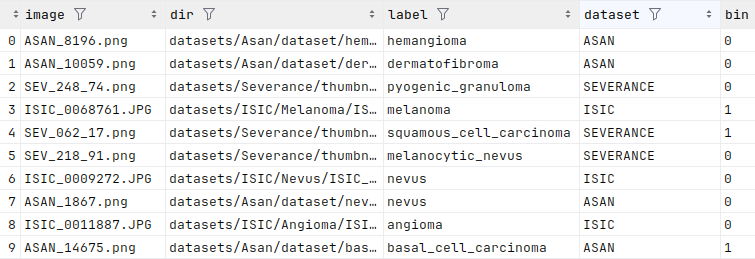
\includegraphics[scale = 0.55]{imagenes/formatocsv.png}
	\caption{Formato del fichero csv normalizado}
	\label {formatocsv}
\end{figure}

Una vez establecido el formato común, podemos pasar al análisis y adaptación propia de cada conjunto.

\subsection{ISIC Dataset}

El dataset ISIC es el mayoritario de la lista, ya que posee casi 60.000 imágenes de alta resolución, del total de casi 108.000 imágenes de las que disponemos. Para su descarga, se han empleado la galería de la web oficial \cite{isicarchive}, donde podemos filtrar cómodamente las enfermedades que queremos descargar. Como criterio de descarga, se han tenido en cuenta únicamente aquellas fotografías correctamente diagnosticadas, ya que existe un total de 27896 imágenesno etiquetadas dentro del repositiorio, las cuales descartaremos. El problema se centrará en resolver un problema de aprendizaje supervisado, por lo que las imágenes no etiquetadas suponen una complejidad adicional y un ruido para el modelo.

Cada clase descargada, además, se ha sometido a un proceso de filtro, sobre todo por cuestiones numéricas; existen nuevas clases, con escasas cantidades de datos, las cuales poseen menos de 10 imágenes, cantidad insuficiente a la hora de clasificar frente a clases como lunares comunes, que tienen en total 32697 ejemplares. De esta forma, nos queda el siguiente conjunto de clases:
\begin{itemize}
	\item Nevus
	\item Seborreic keratosis            
	 \item Actinic keratosis            
	\item Pigmented benign keratosis         
	\item Solar lentigo                           
	\item Dermatofibroma                          
	\item Vascular lesion                         
	\item LIchenoid keratosis                     
	\item Acrochordon                             
	\item Lentigo NOS                             
	\item Atypical melanocytic proliferation       
	\item Aimp                                     
	\item 	Wart                                     
	\item Angioma                                  
	\item Lentigo simplex                          
	\item 	Neurofibroma                             
	 \item 	Scar 
\end{itemize}

Estas clases se almacenan en ficheros zip cada una, así que tras ser descargadas, deben ser extraídas y añadidas al fichero csv que definimos anteriormente. Al tratarase del primer subconjunto que se añadirá, será la parte del código encargada de crear el fichero y establecer las columnas mencionadas. Además, se realizará la transformación de las etiquetas, dispuestas en el formato de la enumeración anterior, a notación snake case. Numerando el proceso, se ha creado un script de python que realiza las siguientes tareas:

 
 \begin{algorithm}[H]
 	\label{extract}
 	\caption{Algoritmo de descompresión de fotografías por carpetas}
 	\begin{algorithmic}[1]
 		
 		\Procedure{extractISIC}{path}
 		\Comment{Obtener una lista de todos los archivos ZIP}
 		 		\State archivosZip : list of strings
 		 		
 		\ForAll{file in path where file.name endswith('zip')}
 			\State archivosZip.add(file)
 		\EndFor

		\Comment{Iterar sobre cada archivo ZIP}
			\ForAll{archivo in archivosZip}
			\State var rutaArchivoZip  $\gets$ join(path, archivo)
			\State var carpetaSalida = path.splitext(rutaArchivoZip).get(0) \Comment{ Eliminar la extensión}
		
			\If {not exists(carpetaSalida)}
				\State makedir(carpetaSalida) 

			\Comment{  Extraer el contenido del archivo ZIP en la carpeta de salida}
			\State \Call{openZipFile}{rutaArchivoZip} as zipRef
			\State zipRef.extractall(carpetaSalida)
			 \EndIf
		\EndFor
 		\EndProcedure
 		
 	\end{algorithmic}
 \end{algorithm}
 
 


\begin{enumerate}
	\item Extraer las imágenes mediante uzip en una carpeta con el mismo nombre de la clase a la que pertenecen \ref{extract}
	\item Crear un fichero .csv, denominado preprocessedData.csv, donde se alojarán las 5 columnas: images, dir, label, dataset, bin.
	\item Recorrer cada carpeta creada, y añadir los 4 primeros campos
	\item Una vez añadidas todas las imágenes, se renombran las etiquetas a camel case mediante las funciones upper(), lower() y replace() de la clase string de python.
\end{enumerate}

\begin{algorithm}[H]
		\caption{Algoritmo de creación del csv}
		\label{isiccrear}
		\begin{algorithmic}[1]
			
		\Procedure{crear\_csv}{path, clases, nombre\_dataset}
		\Comment {Inicializa una lista vacía para almacenar la información de los archivos}
		 \State var info\_archivos : list of strings
		 \State i  $\gets$ 0
		
		 \For{nombre\_carpeta in dir(path)}
			\State ruta\_carpeta $\gets$join(path, nombre\_carpeta)
			
			\If{path.isdir(ruta\_carpeta)}
		
				\Comment {Itera sobre cada archivo en la carpeta}
				\For{nombre\_archivo in listdir(ruta\_carpeta)}
						  \State ruta\_archivo $\gets$ join(ruta\_carpeta, nombre\_archivo)
					\If {isfile(ruta\_archivo) and nombre\_archivo.ends() != "jpg"}
						\State var info\_archivos.add(nombre\_archivo, ruta\_archivo, clases[i], nombre\_dataset)
					\EndIf
					\State i = i + 1
				\EndFor
		 	\EndIf
		\EndFor		
		
	
		\State ruta\_archivo\_csv $\gets$ 'preprocessedData.csv'	\Comment{ Define la ruta del CSV}
		
		\State open(ruta\_archivo\_csv) as archivo\_csv
		 \State archivo\_csv.writerow(["image", "dir", "class", "dataset"])  
		 \Comment{Escribe la cabecera}
		 
		 \EndProcedure
	\end{algorithmic}
\end{algorithm}

Para facilitar el procesado, el rellenado de los datos se realiza sobre una estructura tabular de pandas, para así transformar la columna label fácilmente.
En cuanto a la quinta columna, la clase binaria, dicha tarea se realizará cuando todos los datasets estén añadidos al .csv, de forma que el recorrido de los datos sólo se realice una vez, cuando tengamos disponible todas las clases. 

En cuanto al estudio estadístico de los datos, este se realizará una vez dividido los datos en los conjuntos de entrenamiento y test, definido en entradas posteriores.

\subsection{ASAN}

ASAN es uno de los dos datasets cuyo formato de entrega de los datos consistía en una matriz de imágenes en un canvas de gran resolución. En el caso de este dataset, tenemos un total de 32 imágenes de este tipo, cuya etiqueta se encuentra escrita en el nombre del fichero.
El procesado de este dataset será más complejo que el anterior, ya que debemos recortar cada una de las imágenes, evitando que queden bordes blancos que puedan perturbar la predicción, y sesgar el aprendizaje.

Podríamos idear una solución codificada de forma estricta en la cual la imagen se subdivida en n filas y m columnas para extraer las fotografías; sin embargo, cada uno de los canvas del datasets tiene un número filas y columnas concreto que dificultaría esta tarea de forma automática. En su lugar, se ha medido mediante una herramienta de recorte fotográfico el tamaño de una de las miniaturas, siendo este de 98 píxeles, y será el valor que utilizaremos a la hora de realizar el recortado.

No se debe pasar por alto que las imágenes se encuentran separadas vertical y horizontalmente por espacios en blanco, cuya distancia es variable. Es el factor causante de la imposibilidad de partición regular, por lo que se emplearán técnicas de visión mediante la librería OpenCV para la detección de bordes:

\begin{enumerate}
	\item Eliminar 4 píxeles en blanco de los extremos para que todas las bandas blancas queden del mismo grosor
	\item Hallar el numero de imágenes por fila y columana de forma aproximada, teniendo en cuenta el tamaño de miniatura y el borde.
	\item Recortar la imagen usando el método findContours() de openCV. Este método binaria la imagen transformándola a blanco y negro, y trazado con técnicas de detección de puntos de interés en imágenes los bordes de cada una de las miniaturas, y devolviendo las coordenadas de sus equinas en un vector multidimensional. 
	\item Para cada imagen, obtenemos la esquina superior izquierda de la imagen, y mediante el ancho y alto de la imagen, recortamos dicha sección de la imagen y se almacena en una nueva variable.
	\item Se recortan los bordes de dicha imagen y se almacena el resultado en disco, en una carpeta que posee el mismo nombre que la imagen de la que fue extraída.
	\item Se repite el paso 3-6 para cada imagen de la matriz, pasando a abrir la siguiente matriz hasta que no quede ninguna por recortar.
\end{enumerate}

\begin{algorithm}[H]

		\caption{Recorte de las imágenes de ASAN mediante OpenCV}
		\label{cortarasan}
		\begin{algorithmic}
			\Procedure{recortarImagenesASAN}{path, i, title='ASAN'}
			\State var files : list of strings
			
			 \For {f in pathlib.Path().iterdir()}
			 	 \If {f is\_file()]}
			 	 	\State files.add(f)
			 	 \EndIf
			 \EndFor
			 	 
			\State var names : list of strings
			\State var  diss\_class : list of strings
			 \State var i $\gets 0$
			
			\ForEach {f in files}
				   \State name $\gets$ str(f)[str(f).rfind('\#') + 1:-4]
				   \If {f.ends = 'png' and not exists(path)}
						\State {makedir(name)}
						\State var image = cv2.imread(str(f), cv2.IMREAD\_UNCHANGED): image
						\State var gray = cv2.cvtColor(image, cv2.COLOR\_BGR2GRAY) : image
			
						\State var kernel = cv2.getStructuringElement(cv2.MORP H\_RECT, (5, 5))
						\State var gradient = cv2.morphologyEx(gray, cv2.MORPH\_GRADIENT, kernel)
			
						\State var contours $\gets$ cv2.findContours(gradient, cv2.RETR\_EXTERNAL, cv2.CHAIN\_APPROX\_SIMPLE)
			
						\ForEach{cnt in contours}
								\State	x, y, w, h  $\gets$ cv2.boundingRect(cnt)
								\State var box\_image = image[y: y + h, x: x + w] : image
				
								 \Comment{Recorta la imagen para eliminar el borde} 
								\State var img\_sin\_borde = box\_image[grosor\_borde:-grosor\_borde, grosor\_borde:-grosor\_borde]
								\State cv2.imwrite(f"{name}/{title}\_{i}.png", img\_sin\_borde)
					
								\State names.append(f"{title}\_{i}.png")
								\State diss\_class.add(name)
								
								\State i = i + 1
						 \EndFor
				\EndIf	 
	\EndFor
				
\EndProcedure
\end{algorithmic}
\end{algorithm}

Una vez finalizado el proceso, el proceso a aplicar es similar a ISIC; pero, en este caso, en lugar de simplemente convertir a camelcase, debemos de cambiar los nombres por completo para no usar el formato por abreviaturas original, y poder hacer merge de las clases de este dataset con ISIC que sean de la misma enfermedad. Para ello, simplemente se crea un diccionario clave-valor, donde la clave es el nombre que deseamos cambiar, y el valor, el nuevo nombre. Mediante pandas \cite{reback2020pandas}, el proceso de sustitución se puede hacer de forma inmediata mediante la función replace.

Es importante destacar que el dataset Hallym, también será incluido en el conjunto final, siendo el procedimiento de preprocesado a aplicar exactamente el mismo al descrito en este punto.

\subsection{PAD UFES 20}

PAD UFES 20, como ya describimos en el apartado de Estado del arte, se trata de un dataset diseñado para el entramiento de sistemas de asistencia en diagnóstico computado, donde el experto dermatólogo puede utilizarlo como un medio de apoyo. Contiene 6 enfermedades distintas, siendo 3 cancerosas (células basales, células escamosas o melanoma maligno) y 3 benignas (actinic keratosis, nevus, keratosis seborreica).

La estructura de presentación de los datos es más sencilla que ASAN, pues las imágenes son individuales, y cuentan con un fichero .csv donde se describen las etiquetas y otros metadatos asociados a las imágenes. La única modificación necesaria es actualizar el path de cada imagen y la nomenclatura del diagnóstico de la enfermedad, teniendo en cuenta que debemos de tranformar de abreveviatura a camel case:
\begin{itemize}
	\item NEV $\rightarrow$ nevus
	\item SEK  $\rightarrow$ seborreic\_keratosis 
	\item ACK $\rightarrow$ actinic\_keratosis  
	\item BCC $\rightarrow$  basal\_cell\_carcinoma           
	\item SCC $\rightarrow$ squamous\_cell\_carcinoma
	\item MEL $\rightarrow$ melanoma
	         
\end{itemize}



\begin{algorithm}

	\caption{Formato de las imágenes de PAD UFES}
	\label{cortarpadufes}
	\begin{algorithmic}
		\State  var PAD\_UFES\_PATH : directory of PAD UFES 20 dataset
		\State dict $\gets$ \{'BCC': 'basal\_cell\_carcinoma', 'SEK': 'seborreic\_keratosis', 'SCC': 'squamous\_cell\_carcinoma', 'NEV': 'nevus',
			'ACK': 'actinic\_keratosis', 'MEL': 'melanoma'\}
		\Procedure{preparar\_padufes}{}
		\State df\_pad\_ufes $\gets$ file.read()
		\State  df\_pad\_ufes['diagnostic'] $\gets$ df\_pad\_ufes['diagnostic'].replace(dict)
		
		\ForEach{img in df\_pad\_ufes}
			\State df\_pad\_ufes['im\_dir'] $\gets$  PAD\_UFES\_PATH + '/images/ + img
		   \State df\_pad\_ufes['dataset'] = 'PAD\_UFES'
	
	\EndFor		
		\EndProcedure
	\end{algorithmic}
\end{algorithm}

De esta forma, podemos simplemente hacer fusión de las nuevas filas con el fichero anterior en modo de apertura ``append''.

\subsection{PH2}

Este dataset recoge imágenes provenientes del Servicio de Dermatología del Hospital Pedro Hispano (Matosinhos, Portugal), que recoge pruebas cutáneas realizadas con el sistema Tuebinger Mole Analyzer, y un aumento de 20x. Recordando lo analizado en el capítulo anterior, consta de 200 imágenes dermatoscópicas de lesiones melanocíticas, incluidos 80 lunares comunes, 80 nevus atípicos y 40 melanomas, en una resolución de 768x560 píxeles. La base de datos PH² incluye anotaciones médicas de todas las imágenes: segmentación médica de la lesión, diagnóstico clínico e histológico, y evaluación de varios criterios dermatoscópicos. Entre ellos, encontramos distinción por colores; formación del tejido; puntos/glóbulos; rayas; áreas de regresión; velo azul blanquecino (pgimentación difusa).

Los datos se organizan en directorios de carpetas de varios niveles,  pudiendo encontrar en su interior la imagen dermoscópica, la plantilla de segmentación y regiones de interés de la imagen destacadas mediante una plantilla binaria. Para este trabajo, sólo se utilizarán las imágenes correspondientes al directorio de datos dermoscópicos, ya que con debido a la cercanía de la lensión, la imagen contiene en su mayoría solo información útil.

Como preprocesado de las imágenes, al disponer de ellas correctamente clasificadas en carpetas y con un fichero de metadatos bastante completo, el único procedimiento necesario sería la adición al fichero preprocessedData.csv, realizando las conversión a camel case de las labels. El método a emplear es equivalante al utilizado en PAD UFES \ref{cortarpadufes}.

 \subsection{Severance}
 
 Este dataset, como ya se comentó, provinene del hospital Severance, y el dataset con mayor cantidad de patologías identificadas de la lista. El formato de este repositorio sigue una estructura similar a la de ASAN: las imágenes están organizadas en varias páginas de gran tamaño, donde, a diferencia de ASAN, podemos encontrar varias imágenes por lesión separadas entre cuadros blancos, que contienen escritos en él, la etiqueta de las siguientes imágenes leídas de izquierda a derecha, y de arriba a abajo, hasta encontrar el siguiente cuadro en blanco con texto.
 
 La dificultad de este preprocesado radica precisamente en la existencia de los cuadrados blancos, ya que la lectura del texto escrito en ellos es prácticamente imposible. La baja resolución, unido a la existencia de etiquetas cuyo nombre se encuentra dividido en varias líneas, provoca que algoritmos de reconocimiento de texto como Pytesseract \cite {pytesseract} no fuesen capaces de detectar las etiquetas adecuadamente.
 
 Por este motivo, fue necesario identificar manualmente cuántos casos de cada enfermedad existían por matriz de imágenes, y realizar un recuento para saber cuándo aplicar una etiqueta u otra. Conociendo que las etiquetas asignadas aparecían por orden alfabético, el proceso a seguir se resumió en aumentar un contador cada vez que aparecía una imagen en blanco durante el recorrido de las imágenes, y aumentar el contador hasta llegar al valor total de ejemplares de esa clase; en ese momento, se procede a contar los valores de la siguiente. Con este procedimiento, nos queda el algoritmo 3.5(\ref{fig:cortarseverance})
  
La ventaja respecto a ASAN reside en que los espacios en blanco entre imágenes tienen el mismo grosor, y fue posible de separar en submatrices sin necesidad de utilizar ténicas de visión, que ralentizan el proceso extracción. Cada imagen es etiquetada siguiendo el formato establecido  y siendo añadida a una nueva carpeta, desde la cual se referenciarán mediante el fichero preprocessedData.csv. 

Como dificultades a destacar durante el desarrollo de este procedimiento, comentar que la detección de la imagen en blanco que separa las etiquetas entre clases no es trivial. El método elegido para distinguirla es emplear un  umbral de número de píxeles con valor de escala de grises blanco, es decir, 255. El valor de dicho umbral se calculó de forma experimental , ya que si el valor era demasiado bajo, pieles sanas o de color claro también cumplían la restricción. El cambio de etiquetado no se produce si el número de píxeles totales de la imagen encontrada no supera un valor x de miles de píxeles. De forma experimental, el valor 20.000 fue el que mejor resultados aportó, funcionando en todos los casos.

Aumentar de forma desmesurada este valor también puede tener consecuencias negativas, ya que el nombre de la etiqueta se encuentra escrita en la parte inferior de estas imágenes y aportan píxeles de color negro que no cumplirían la condición.


 \begin{algorithm}[H]
	\label{fig:cortarseverance}
	\caption{Recorte de las imágenes de Severance mediante OpenCV}
	\begin{algorithmic}
		\Procedure{recortarImagenesSEVERANCE}{path}
		
		\State  df\_sev $\gets$ read('SeveranceA.xls')
		\If {not os.path.exists('thumbnails')}
		\State makedir('thumbnails')
		\EndIf
		
		\State var files : list of strings
		
		\For {f in pathlib.Path().iterdir()}
		\If {f is\_file()]}
		\State files.add(f)
		\EndIf
		\EndFor
		
		\State var names : list of strings
		\State diss\_class : list of strings
		\State j $\gets 0$
		
		\For {f in files}
		\If {f.ends = 'jpg'}
		\State name $\gets$ f.name[0:-4]
		\State {makedir(name)}
		\State var image = cv2.imread(name, cv2.IMREAD\_UNCHANGED): image
		\State var image\_split = $\begin{matrix}
			[ image_1 image_2, \ldots, image_8 ] \end{matrix}^T$	\Comment{División por filas}
		
		
		\State var i $\gets$ 0
		
		\ForEach{im  in image\_split}
		\Comment{Recorta la imagen en columnas}
		\State image\_split\_col = np.split(im[:, 2:-3], 15, axis=1)
		\ForEach {imcol in image\_split\_col}
		\State img\_sin\_borde$\gets$ imcol[grosor\_borde:-grosor\_borde, grosor\_borde:-grosor\_borde]
		\If {np.count\_nonzero(imcol == 255) > 20000)}  \Comment{Si es imagen de separador con nombre}
		\State j $\gets j + 1$  \Comment {Cambiamos de etiqueta al siguiente paciente}
		\State continue
		\Else
		\State actual  $\gets$ df\_sev.get(j)
		
		\State	actual.add('{name}\_{i}.png')
		\State	trainProcessed.add(actual)
		\Comment{Guardamos la imagen y añadimos su nombre}
		\EndIf
		\State cv2.imwrite(f'thumbnails/{name}\_{i}.png', img\_sin\_borde)
		\State names.append(f"{name}\_{i}.png")
		\State i $\gets i + 1 $
		
		\State diss\_class.add(name)
		\EndFor
		
		\EndFor
		\EndIf	 
		\EndFor
		\State trainProcessedDF.write("severanceTrainingSet\_thumbnails.csv") \Comment{Guardado en disco}
		\EndProcedure
	\end{algorithmic}
\end{algorithm}
 
 \subsection{Etiquetado binario}
 
Una vez disponemos de todas las imágenes correctamente etiquetadas y redireccionadas desde el fichero preprocessedData.csv, podemos continuar con el etiquetado binario de las enfermedades. Para disponer también de los datos de malignidad de las enfermedades, se ha realizado manualmente una distinción de las distintas enfermedades entre benignas y malignas. Debido a la minoría de imágenes por defecto, para reducir el tamaño del diccionario de enfermedades, por defecto se establecieron todas las etiquetas por defecto a 0, y aquellas pertenecientes al subconjunto de malignas, a 1, siguiendo el siguiente procedimiento:
 
 \begin{enumerate}
 	\item Crear una nueva columna, de nombre ``bin'', que contendrá 0 como valor de inicialización.
 	\item Construir un diccionario o lista con aquellas enfermedades que son malignas.
 	\item Se recorre la columna target para comparar la enfermedad del ejemplar con la lista de enfermedades malignas. En caso de ubicarse en ella, se cambia el valor de ``bin'' por un 1.i
\end{enumerate}

De esta forma, obtenemos la quinta columna, expresada con ceros y unos. Dependiendo de la función de pérdida y el framework posteriormente utilizado, estas etiquetas tendrán que ser categóricas, pero dicho paso puede realizarse de forma inmediante con un casting de tipos, o bien, un el uso de la función replace de python ya mostrada en la fase de homogeneización de los datos.



\begin{figure}[H]
	\centering
	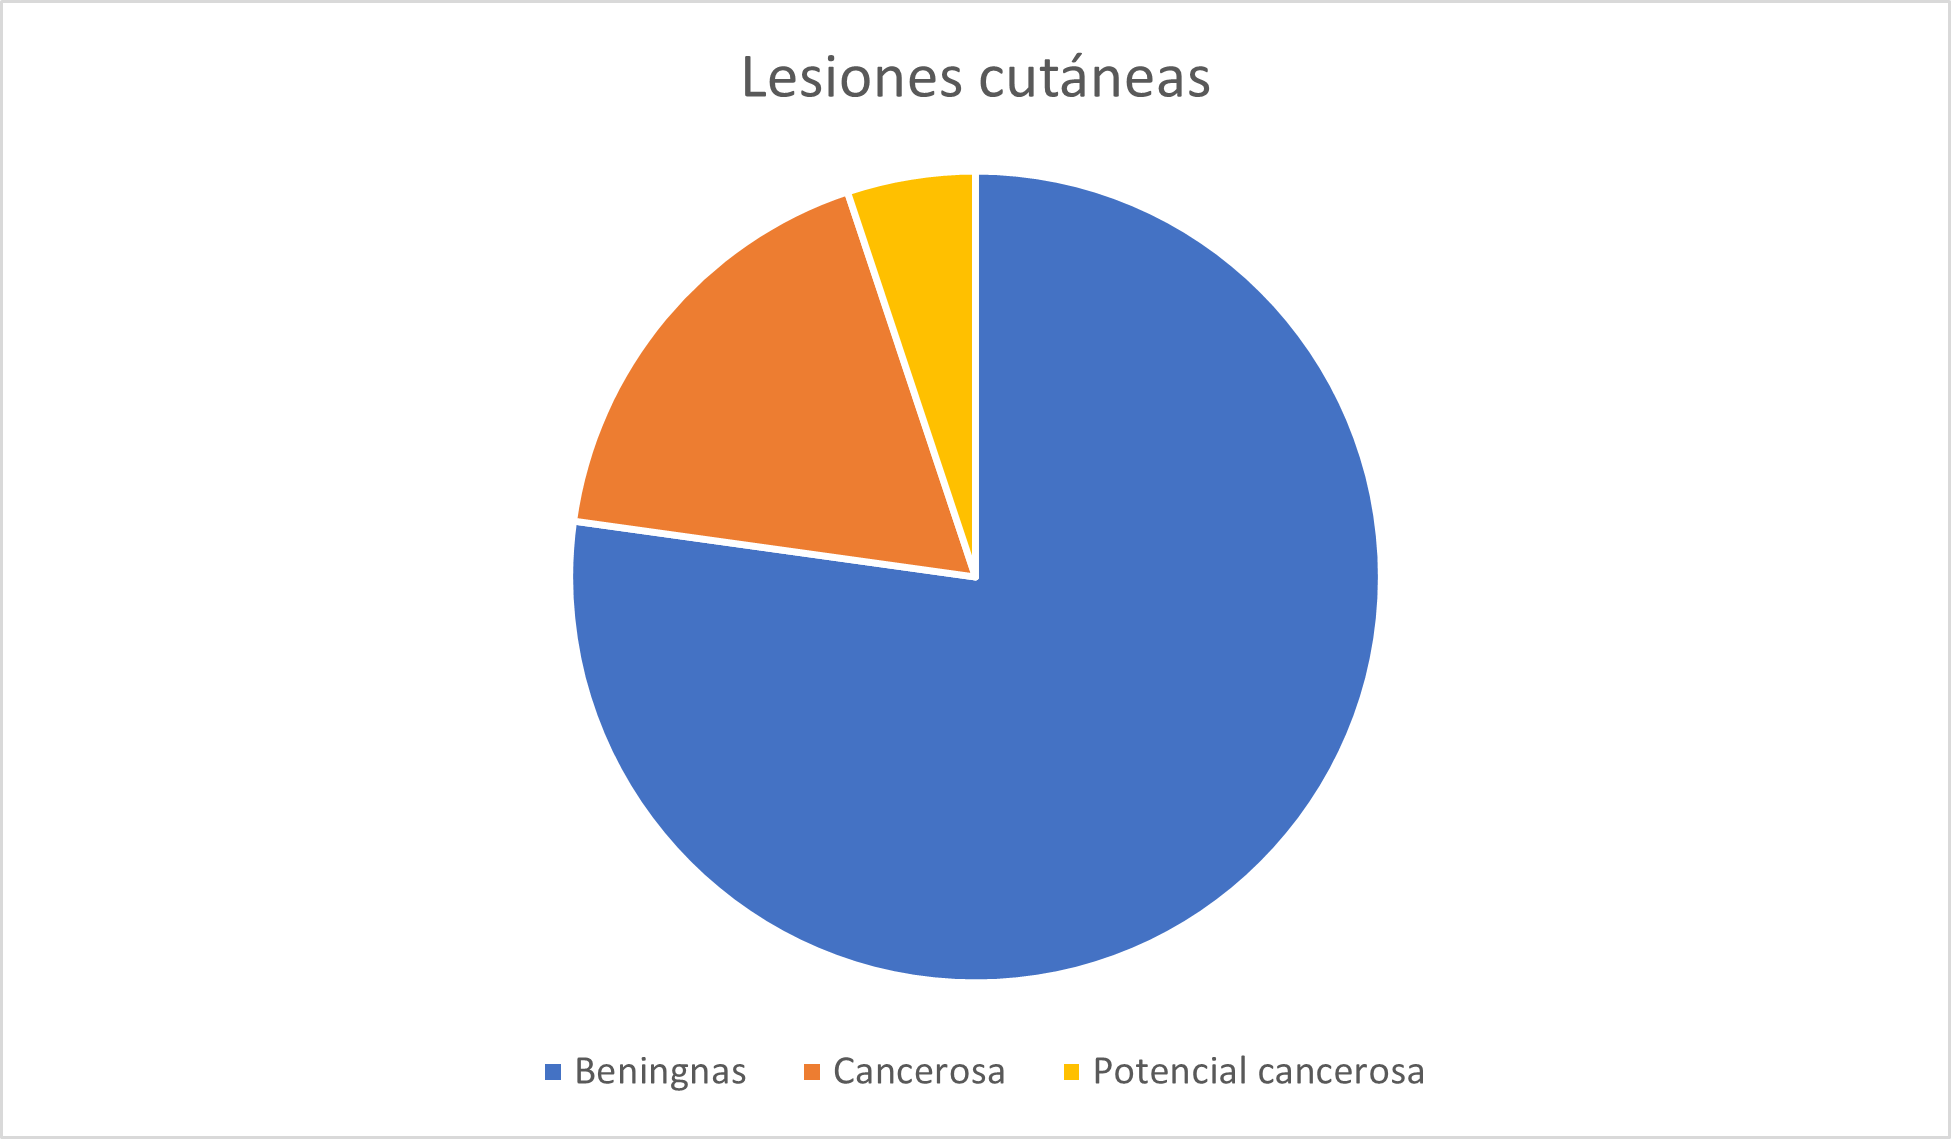
\includegraphics[scale = 0.7]{imagenes/datasetfinal.png}
	\caption{Distribución de clases}
		\label {tartabinaria}
\end{figure}

Si agrupamos por lesiones benignas, cancerosas, y potencialmente cancerosas, podemos obtener el siguiente diagrama de sectores de la figura \ref{tartabinaria}, donde se puede observar cómo la mayoría de imágenes disponibles engloban problemas de piel no cancerosos, mientras que el segundo tipo más común de lesión si es la cancerosa. Las lesiones potenciales, como ya se comentó, pasan a formar parte de las lesiones benignas debido a que en el momento de la captura, continúan siendo benignas.

Con este paso, finalizamos la uniformización de los datos en lo que corresponde al formato del etiquetado y gestión de directorios. A continuación, se realizarán las fases de partición de los datos, y de preprocesado de la imagen en sí, empleando como referencia el estudio realizado en el estado del arte.


\section{Particionado de los datos}

En este punto, estudiaremos la importancia de un correcto particionado de los datos para el entrenamiento del modelo y su posterior verificación de rendimiento. Se estudiará la importancia de disponer de un estimador insesgado del modelo entrenado, y las decisiones tomadas para el problema que nos concierne en lo que respecta a la calidad de imagen. Para su mejora en calidad, emplearemos GANs con las imágenes de inferior resolución.

\subsection{Importancia de la separación train-test}
En las tareas de aprendizaje de Machine learning y Deep learning, el objetivo es disponer del mayor número de datos posible, por lo que la opción de privar al proceso de entrenamiento de un subconjunto de ellos, o incluso proceder a su eliminación, puede ser una decisión demasiado drástica que ha de tomarse con fundamento.\\

Sin embargo, cuando realizamos un modelo de aprendizaje, realmente estamos creando una hipótesis, un modelo que construimos y queremos hacer que se acerque lo máximo posible a la expresión que define la población real del problema. Pero, para poder estimar la bondad de nuestro ajuste de forma fiable, necesitamos algún estimador no sesgado que nos indique la calidad del modelo, que nos permita saber el error que comete nuestra hipótesis con respecto a la distribución de la población real, al que denominaremos como error fuera de la muestra, abreviado como $E_{out}$.  Esto se debe a que, para construir este modelo aproximado, estamos empleando una muestra de la población, la cual es continuamente iterada para ir ajustando los filtros aplicados sobre el conjunto y que permite inferior de sus características extraídas las etiqueta de cada una de las imágenes.\\

Podemos conseguir un estimador insesgado separando un conjunto de datos del total, y obteniendo un conjunto de test, el cual no se ha visto involucrado en ninguna fase del proceso de aprendizaje. La hipótesis final, a la que llamaremos $g$, es evaluada en este subdataset, y el resultado será un buen estimador del $E_{out}$. A este error podemos llamarlo $E_{test}$. Al seleccionarlo como estimador de $E_{out}$, estamos afirmando de alguna manera de que éste se tratará de un estimador que generaliza muy bien el error out-of-sample.\\

Este conjunto recibirá un número efectivo de hipótesis $|\mathcal H|= 1$, es decir, únicamente es evaluado con la hipótesis final de nuestro modelo (su ajuste paramétrico final). Esta hipótesis se elige sin conocer el comportamiento de los datos que el conjunto de test contiene, ya que si la estimación de $g$ se ve afectada de alguna forma por los ejemplares ya utilizados en el entrenamiento, no conseguiremos un estimador insesgado, y la ecuación de Hoeffding, no será aplicable. Dicha ecuación enuncia, que para muestras idénticamente distribuidas, e independientes entre sí, se cumple la siguiente desigualdad \cite{Mostafa2012}:

$$P(\mathcal{D}: | E_{out}(h) E_{in}(h) |  > \epsilon \leq 2e^{-2\epsilon^2	N}$$

Donde, para cualquier valor de $\epsilon$:
\begin{itemize}
	\item $\mathcal{D}$ es el nombre que recibe el conjunto de entrenamiento.
	\item $ E_{out}$ es el error out-of-sample, error teórico con respecto a distribución real de los datos.
	\item  $E_{in}$ es el error in-sample, es decir, el error cometido durante el proceso de entrenamiento entre las etiquetas inferidas, y su valor real, también conocido como y verdadero.
	\item $N$ es el tamaño de la muestra de datos disponible.
\end{itemize}

Es decir, se cumple que $E_{out}$ se convierte en un estimador muy cercano al valor real del modelo. Dichas restricciones de independencia y pertenencia a la misma distribución son claves,
 motivo por el cual la eliminación de imágenes duplicadas fue clave (ya que cualquier contaminación entre el conjunto de entrenamiento y aprendizaje puede crear sesgos al alza en los resultados). \\

El valor del entrenamiento $E_{in}$ sí que sería un estimador sesgado de forma optimista, pues el modelo ha adaptado los filtros para ser capaz de inferior el mayor número posible de etiquetas correctas del conjunto de entrenamiento.. Pero esto no ha ocurrido con test, por lo que podemos dar como resultado un estimador fiable y robusto de cómo se comportará nuestro modelo con otros elementos de la población real.\\

Cuanto mayor es el tamaño del conjunto, más cercano será el valor del error de nuestra partición de test, $E_{test}$, con respecto a $E_{out}$. Pero, cuantos menos datos para entrenar dispongamos, menos se parecerá la estimación al comportamiento real de la población, y a $f$. Tenemos que conseguir un equilibrio entre ambos tamaños para aprovechar la mayor cantidad de datos posibles, pero disponiendo de un $E_{test}$ fiable. Normalmente, los valores recomendados suelen ser entre un 10\%-30\% de porcentaje de los datos dedicados al conjunto de test, quedando entre un 70-90\% de datos de entrenamiento. Para este problema, la separación entrenamiento-test elegida ha sido 60-40, respectivamente, que a priori, puede ser muy elevada y salir de la recomendación empírica, pero debido a la existencia de grandes desiquilibrios y una cantidad de datos más que suficiente, de aproximadamente 110.000 ejemplares, podemos obtener de esta forma un estimador muy fiable.\\

A continuación, se realizará todo el proceso de separación de datos, entre entrenamiento y test en proporción 60-40. Aunque, idealmente, este proceso de hace de forma completamente aleatoria y sin intervención, he optado por realizar la separación de forma estratificada. Esto hace referencia al mecanismo de separación de los datos teniendo en cuenta el conteo de cada una de las clases. Lo que he realizado ha sido, en primer lugar organizar los datos por sus respectivas clases, dentro de cada dataset, de forma que se tienen dos vectores cuyo contenido son las tuplas de cada clase por separado. 

Pero este aspecto no solo se da a nivel de subdataset, sino también a nivel del dataset global; es importante tomar una cantidad proporcional de cada clase para evitar que el algoritmo sesgue sus resultados al encontrar patrones comunes propios de cada subconjunto, y este no sea capaz de aprender la visión general de los elementos que definen a un tipo de lesión concreto. Por tanto, definiré un ``doble nivel de estratificación'', donde:

\begin{enumerate}
	\item A nivel de cada subdataset, extraer mediante partición estratificada un porcentaje de entrenamiento, y otro de test en proporción 60-40 a la hora entrenar.
	\item Volver a unir las clases de entrenamiento de cada dataset, y test de cada dataset, en los dos ficheros que comprenderán las imágenes asociadas al conjunto de entrenamiento y al conjunto de test.
\end {enumerate}

De esta forma, podemos conseguir proporcionalidad entre dataset y entre clases entre train y test, y hacer que la distribución de las imágenes sea prácticamente la misma. Aunque normalmente se suele realizar la separación de forma completamente aleatoria, en clasificación podría darse el caso extremo en el que una clase completa no aparezca en el conjunto de entrenamiento, y nuestro modelo obtenga pésimos resultados de $E_{test}$.  Si bien la probabilidad es muy baja, matemáticamente puede suceder estadísticamente hablando, y consideramos que no afecta negativamente al análisis haber realizado la partición de forma proporcional a cada clase y dataset.

Comentando en detalle la implementación realizada, es de interés destacar el empleo de la función train-test split de SKlearn \cite{scikit-learn}. Se trata de una función que realiza de forma bastante simplificada el proceso de partición estratificada. En este caso, además, se verificará la existencia de clase con menos de 16 ejemplares de imagen presentes para confirmar que no se han filtrado clases minoritarias las cuales son imposibles de clasificar con el modelo actual. El resultado es el código de la figura \ref{fig:separar}

 \begin{algorithm}[H]
	\caption{ Separación de las filas según el valor de la columna ``column''}
		\label{fig:separar}
	\begin{algorithmic}
		\State MIN\_COUNT = 16
		\Procedure{separar\_subdata}{dataframe, column}
		\State var separated $\gets$ dataframe $\matrix{[c_1, c_2, \cdots, c_n]} / c_{i _j}= column$ y $separated[k] \cap separated[l] = {0}$ para $k\neq l$
		\State var trainData, testData: list of tuples
		\State lista\_elementos: array of tuples
		
		\ForEach{ data\_part, contenido in separated}
			\State lista\_elementos = lista\_elementos $\cup$ contenido
			\If { lista\_elementos["class"].map(counts) > MIN\_COUNT}
				\State var train, test = \Call{train\_test\_split}{subdata, test\_size=0.4,seed=19, shuffle=True, stratify=subdata['class']}
				\State  trainData = trainData $\cup$ train
				\State  testData = testData $\cup$ test
			\EndIf
		\EndFor \\
	\Return lista\_elementos
		
		\EndProcedure
		
	\end{algorithmic}
\end{algorithm}

De esta forma, seguimos manteniendo la proporción a nivel de conjunto global, y de subdataset. En caso de necesitar entrenar únicamente con uno de los subconjuntos añadidos, podemos filtrar el cojunto de tuplas por aquellos cuya clase sea igual a la buscada.

\subsection{Particionado de validación}

Una vez separado nuestro conjunto de test, únicamente trabajaremos con el resto de valores, que componen el conjunto de entrenamiento. Con ellos, realizaremos el estudio estadístico, ya descrito parcialmente en el punto anterior, y todo el procedimiento de preprocesado de imágenes y ajuste del modelo.

Durante las fases de ajuste del modelo elegido en nuestras hipótesis, necesitaremos estudiar qué parámetros favorecen mejores resultados, así como el tipo de regularización a emplear y el coeficiente $\lambda$ de participación de este.

Una forma de realizar esta práctica consiste en el uso del subconjunto de validación. Este concepto se asemeja al concepto del conjunto de test, con la diferencia de que se utiliza como estimador insesgado para evaluar los parámetros relevantes de cada algoritmo, o los modelos a comparar. Estimamos el error out-sample de forma directa mediante el error obtenido $E_{val}$. Lo conseguimos al evaluar el modelo sin tener en cuenta los K valores extraídos para la validación, utilizándolo como estimador, $E_{val}$.

$$E_{out}(g) \approx E_{out}(g^-) \approx E_{val}(g^-)$$

Siendo $E_{out}(g)$ el error final cuando se utiliza todo el conjunto de datos $\mathcal D$.
La parte izquierda de la ecuación funciona mejor cuanto más pequeña sea k, mientras que por la derecha, un mayor valor de k permitirá una mejor estimación a traves de $E_{val}$.\\

El caso ideal sería, para acercanos lo máximo posible entre $E_{out}(g)$ y $ E_{out}(g^-)$ es elegir k lo más pequeño posible, cuyo caso extremo es k=1. De esta forma estaríamos haciendo \textbf{leave one out}, método el cual evalua todo el conjunto como entrenamiento, reservando solo un único valor para validación. La combinación de este proceso aplicado a todos los elementos nos permitirá conseguir el error de valicación cruzada, dado por:

$$E_{cv} = \frac{1}{N}\sum^{N}_{n=1} e_n$$

donde $e_n = E_{val}(g^-_n) = e(g_n^-(x_n),y_n)$, tal y como se ha explicado. Pero es muy costoso computacionalmente, sobre todo ante casos como este, donde el conjunto de entrenamiento contiene alrededor de 60000 valores. Es por ello que simplificaremos este enfoque al conjunto de validación único.\\

Un caso menos costoso computacionalmente es $V$ Cross-Validation, donde dividimos todo el conjunto de datos en V subconjuntos, 5 o 10 habitualmente, llamados \textbf{folds}. En este proyecto, donde disponemos de un conjunto considerable de valores, no he considerado conveniente realizar el proceso de Validación cruzada (CV), ya que este consistiría en disponer de varios conjuntos de validación distintos, y entrenar el modelo para cada uno de los conjuntos de datos restantes no pertenecientes a validación. Debido a que los tiempos de entrenamientos de redes convolucionales pueden superar los días y semanas de duración, no permitiría tener en cuenta otros aspectos claves del proyecto más allá del ajuste de parámetros.\\

Los valores escogidos para esta partición será un \textbf{70\% de entrenamiento, y 30\% de validación}.

\section{Uso de GANs de super resolución}

Las imágenes procedentes de los datasets seleccionados poseen una buena resolución, siendo esta, en media, prácticamente equivalente a lo que se conoce como alta resolución en aprendizaje profundo (1024 x 1024). Sin embargo, aquellas imágenes pertenecientes a los datasets Severance y ASAN, que fueron almacenadas en forma de matriz de imágenes, poseen una calidad muy pobre, de apenas 98x98 píxeles, como ya destacamos durante su preprocesado. En caso de que estos datasets aporten clases completamente nuevas respecto a los 3 conjuntos restantes, la red podría clasificarlas erróneamente basándose únicamente en la resolución.\\

Un simple reescalado solo provocaría altas frecuencias en la imagen que colaborarían en la aportación de ruido al modelo. Hacen falta técnicas más avanzadas, que permitan hacer crecer el tamaño de la imagen sin interferir en su estructura conjunta. Una de estas alternativas, es el uso de redes generativas adversarias (GANs).

\subsection{Justificación de uso}

Las redes generativas adversarias (GANs)  \cite{goodfellow2014generative} son una arquitectura de aprendizaje profundo de tipo generativo, cuyo objetivo suele ser la generación de imágenes sintéticas capaces de imitar con un alto grado de confianza un conjunto de imágenes concreto dado como entrenamiento, estudiando su distribución y siendo capaces de generar imágenes capaces de hacerse pasar por las originales.

Se trata de una arquitectura surgida en 2014 del grupo de investigación de Ian Goodfellow \cite{goodfellow2014generative}, cuya arquitectura consiste en el uso de dos redes profundas: la red generadora, y de discriminatoria.

 \begin{itemize}
 	\item La de red generadora genera imñagenes que intentan asemejarse a las proporcionadas como entrenamiento, de forma que estas se hagan pasar por las originales.
 	\item La red discriminativa, infiere si la imagen recibida como entrada es o no verídica, y le transmite dicho valor de confianza a la red generadora, para que ésta sea capaz de ajustarse para mejorar el resultado.
 	\end{itemize}
 	
 Este tipo de arquitectura, basada en la colaboración entre las dos redes, tiene cierta similitud con el aprendizaje con refuerzo, ya que los ajustes a realizar sobre el modelo generador, depende con fuerza del feedback recibido por la función de pérdida de la red discriminativa.\\
 
 Se trata de un proceso comúnmente vinculado al aprendizaje no supervisado, en el que el interés reside en la generación de imágenes sintéticas para fines como el entrenamiento de otros modelos profundos con clases infrarrepresentadas. La GAN puede encargarse de aumentar el tamaño sintéticamente de aquellas clases infrarrepresentadas para mejorar la calidad del aprendizaje y que este se realice de forma equilibrada. Por tanto, puede considerarse como una técnica de aumento de datos.

Sin embargo, esta no se trata de la única aplicación. El problema al que nos enferentamos, donde requerimos un aumento de la resolución para la mejora de calidad de la imagen, también es una tarea realizable y demostrada por la literatura en la que las GANs logran buenos resultados. Al expandir una imagen de tamaño, requerimos ``rellenar'' aquellos píxeles intermedios faltantes al redimensionar la imagen. Ésta tarea es bastante similar a la realizada pora una GAN tradicional, con la diferencia de que sólo debemos generar los píxeles intermedios, y de forma que éstos se adapten al entorno del resto de la imagen.  ESRGAN\cite{wang2018esrgan} logra este efecto.\\

Esta red ha demostrado cuantiosos éxistos en la literatura al ser utilizada como forma de reescalado de datos, debido a sus mejoras propuestas frente a las GANs tradicionales. Una de las claves reside en la función de pérdida; en lugar de discriminar si la imagen es adecuada o no, se ha empleado un "grado de percepción" (Perceptual Loss) de la imagen, donde se discrimina la calidad de la imagen generada en una escala. \\

\begin{figure}[H]
	\centering
	\label {fig:esrgan}
	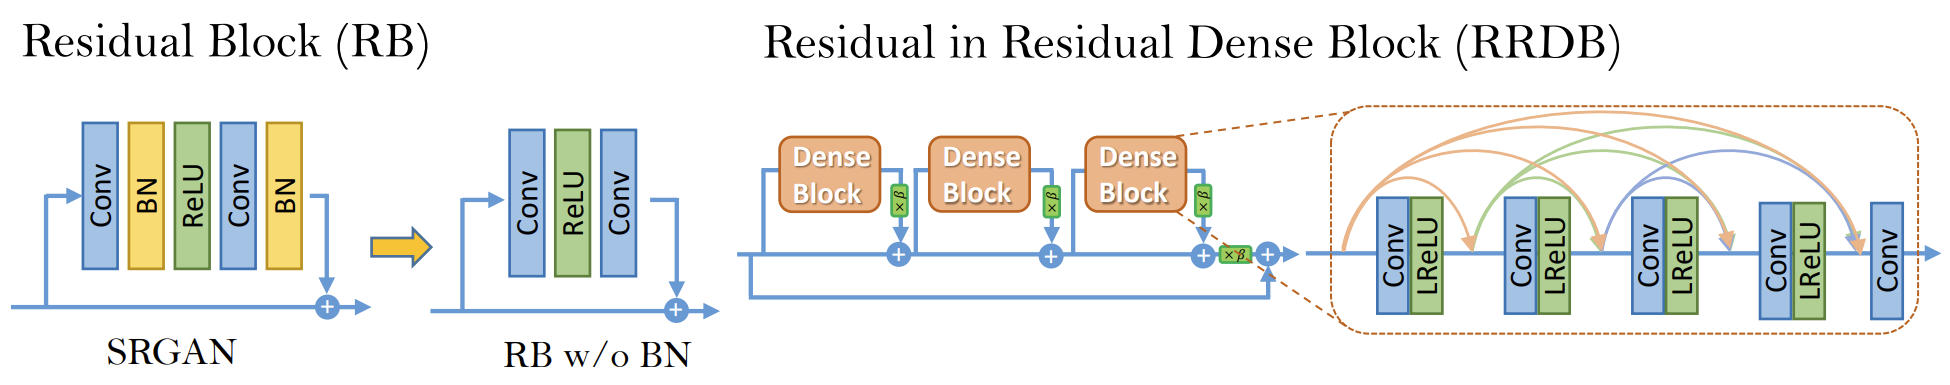
\includegraphics[scale = 0.2]{imagenes/esrgan.png}
	\caption{Arquitectura de ESRGAN. Fuente: \cite{wang2018esrgan}}
\end{figure}


Además, incorpora a la arquitectura las conexiones residuales al estilo de ResNet, con la diferencia de que todos los niveles de un bloque están conectados a todas las siguientes una conexión residual, arquitectura la cual han denominado Residual-in-Residual. Esto les ha permitido evitar la decaída de gradiente, y además, prescindir de la capa de Batch Normalization, que introducía artefactos en el resultado final.

Concluimos que este modelo es el adecuado para el problema, debido a sus buenos resultados a nivel de mejora de imagen, y de sus resultados ya mostrados en modelos de la literatura \cite{healthcare10071183}, donde la aplicación de ESRGAN ofrece mejoras en el resultado del modelo evaluado, siendo este resultado evaluado con distintas arquitecturas y modelos de redes convolucionales del estado del arte.

Gracias a este modelo, el aumento de resolución podrá darse para equiparar la calidad de las imágenes recopiladas.

\subsection{Proceso de reescalado}

La aplicación del proceso de mejora de las imágenes se llevará a cabo únicamente sobre el conjunto de entrenamiento, para así evitar la contaminación del conjunto de test. Podemos encontrar el modelo de ESRGAN ya preentrenado en su repositorio de Github \cite{gitesrgan}.

Dentro del software incorporado para su uso, podemos encontrar el modelo preentrenado para una multiplicación de la resolución a 4 veces mayor. Este será el modelo con aquellos subconjuntos de menor resolución, para así aumentar la resolución de 98x98 a 392x392 píxeles. El procedimiento a seguir ha sido el siguiente:

\begin{enumerate}
	\item Listar las imágenes de entrenamiento pertenecientes a los subconjuntos ASAN y Severance
	\item Aplicar el aumento de resolución, generando las nuevas imágenes en una carpeta nueva
	\item Sustituir las imagenes originales por las aumentadas, conservando las imágenes fuente en un directorio de respaldo.
\end{enumerate}

De forma organizada, nos queda resumido en  el siguiente pseudocódigo:

\begin{algorithm}[H]
	\label{fig:escalar}
	\caption{ Aumento de resolución para ASAN y Severance}
	\begin{algorithmic}
		\Procedure{reescalar\_img}{path\_orig, nombre\_carp}
		\If{not exists(nombre\_carp)}
				\Comment{Renombrar la carpeta a ``nombre\_lr''}
				\State \Call {rename}{path\_orig, nombre\_carp}
				
				\State \Call{mkdir}{path\_orig}
				\Comment{ Creamos carpeta con el nombre original }
				\State \Call {read\_images}{path\_orig + "\_lr", path\_orig}
		\EndIf
		\EndProcedure
		
	\end{algorithmic}
\end{algorithm}

Donde la función 'read\_images' \ref{fig:readimg} es la encargada de recorrer la carpeta, tomar las imágenes y generar su imagen aumentada por super resolución:

\begin{algorithm}[H]
	\caption{ Aumento de resolución para ASAN y Severance}
		\label{fig:readimg}
	\begin{algorithmic}
		\Procedure{read\_images}{path\_orig, nombre\_carp}
		
		\State var im\_path += ``/*''
		\State var model\_path = 'ESRGAN/models/RRDB\_ESRGAN\_x4.pth':path
		\State \Call {load\_model}{model\_pat}
		
		\State var idx $\gets$ 0
		\ForEach {path in im\_path}
			\State idx $\gets idx +1$
			\State var base\_dir= osp.splitext(osp.basename(path))[0] :path

			\State var img = \Call{imread}{path, format = IMREAD\_COLOR}
			\State img = $\matrix     {img} * 1.0 / 255$ \Comment{Normalización antes de aumentar}
			\State img = $img^T.squeeze()$	\Comment{Formato de entrada del modelo }
			\State img\_LR = img.unsqueeze(0).to(GPU)
		
			\State output $\gets model.predict(img\_LR)$
			\State output $\gets$  output,squeeze()
				
			\State output = model(img\_LR).data.squeeze().float().clamp\_(0, 1)
			\State img = $\matrix     {img}^T * 255$ \Comment{Deshacemos cambios}
			 \State Call {imwrite}{f'{im\_out}/' + 'png'.format(base), output)}	\Comment{Guardo en disco}
		\EndFor
		\EndProcedure
		
	\end{algorithmic}
\end{algorithm}

De esta forma, conseguimos reescalar cada una de las imágenes sin necesidad de modificar el archivo .csv previamente guardado para entrenamiento y test. Los resultados son bastante notables, ya que al aumentar la resolución a una 4 veces mayor, pueden apreciarse detalles con mayor claridad \ref{fig:calidad}. 
	
l\begin{figure}[H]
		\centering
		\subfigure[Original]{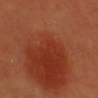
\includegraphics[width=0.3\textwidth]{imagenes/194_13_orig.jpg}} 
		\subfigure[Reescalada]{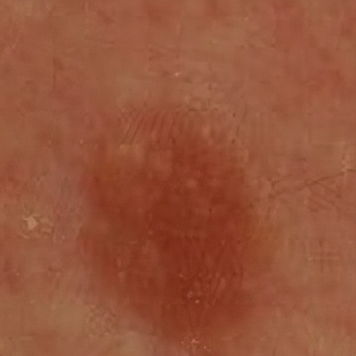
\includegraphics[width=0.3\textwidth]{imagenes/SEV_194_13.png}} 
	\caption{Imagen original (izquierda) vs aumentada (derecha)}
	\label{fig:calidad}

\end{figure}

Como inconvenientes, destacar la gran necesidad de espacio en disco, ya que las imágenes al ser reescaladas y almacenadas en formato sin pérdidas (PNG), han multiplicado el tamaño del dataset completo de entrenamiento en casi 6 veces. Adicionalmente, se han requierido una hora y doce minutos para el reescalado de las imágenes, haciendo uso de una GPU Nvidia Geforce RTX 3080. 


